\title{Estimating Mutual Information from Average Classification Error}
\author{Charles Zheng and Yuval Benjamini}
\date{\today}

\documentclass[12pt]{article} 

% packages with special commands
\usepackage{amssymb, amsmath}
\usepackage{epsfig}
\usepackage{array}
\usepackage{ifthen}
\usepackage{color}
\usepackage{fancyhdr}
\usepackage{graphicx}
\usepackage{mathtools}
\usepackage{csquotes}
\definecolor{grey}{rgb}{0.5,0.5,0.5}

\begin{document}
\maketitle

\newcommand{\tr}{\text{tr}}
\newcommand{\E}{\textbf{E}}
\newcommand{\diag}{\text{diag}}
\newcommand{\argmax}{\text{argmax}}
\newcommand{\Cov}{\text{Cov}}
\newcommand{\Var}{\text{Var}}
\newcommand{\argmin}{\text{argmin}}
\newcommand{\Vol}{\text{Vol}}
\newcommand{\comm}[1]{}
\newcommand{\indep}{\rotatebox[origin=c]{90}{$\models$}}
\newcommand{\Cor}{\text{Cor}}


\begin{abstract}
Multivariate pattern analyses approaches in neuroimaging are
fundamentally concerned with investigating the quantity and type of
information processed by various regions of the human brain;
typically, estimates of classification accuracy are used to quantify
information.  While a extensive and powerful library of methods can be
applied to train and assess classifiers, it is not always clear how to
use the resulting measures of classification performance to draw
scientific conclusions: e.g. for the purpose of evaluating redundancy
between brain regions.  An additional confound for interpreting
classification performance is the dependence of the error rate on the
number and choice of distinct classes obtained for the classification
task.  In contrast, mutual information is a quantity which is in
principle defined independently of the experimental design, and has
ideal properties for comparative analyses.  One obstacle to wider use
of mutual information is the difficulty of estimating mutual
information in high-dimensional neuroimaging data.
%Nonparametric estimators have poor finite-sample performance, and parametric approaches require unrealistic assumptions such as multivariate Gaussianity.
%While one can obtain a lower bound using the mutual information of the confusion matrix, the lower bound obtained is usually quite poor.
We propose a new estimator of mutual information based on the concept
of "average Bayes error."  Under the assumption that the error of a
classifier approximates the average Bayes error, we obtain an estimate
of mutual information based on an asymptotic functional relationship
between average Bayes error and mutual information.  We demonstrate
the utility of our approach in simulated and real data examples.
\end{abstract}


\section{Introduction}

%% YUVAL'S REMIX

A fundamental challenge of computational neuroscience is to understand
how information about the external world is processed and represented
in the brain. Each individual neuron aggregates the incoming
information into a single sequence of spikes--an output which is too
simplistic by itself to capture the full complexity of sensory
input. Only by combining the signals from massive ensembles of neurons
is it possible to reconstruct our complex representation of the
world. Nevertheless, neurons form hierarchies of specialization within
neural circuits, which are further organized in various specialized
regions of the brain.  At the lowest level of the hierarchy--individual neurons,
it is possible to infer and interpret the functional relationship between
a neuron and stimulus features of interest using single-cell recording technologies.
Due to the inherent stochasticity of the neural output, it is natural to
view the neuron as a noisy channel, and use mutual information
to quantify how much of the stimulus information is encoded by the neuron.
Moving up the hierarchy to the the macroscale level of organization in the
brain requires both different experimental methodologies and 
new approaches for summarizing and inferring measures of
information in the brain.

Shannon's mutual information $I(X; Y)$ is fundamentally a measure of dependence
between random variables $X$ and $Y$, and is defined as
\[
I(X;Y) = \int p(x, y) \log \frac{p(x, y)}{p(x)p(y)}dxdy.
\]
Various properties of $I(X; Y)$ make it ideal for quantifying the information between
a random stimulus $X$ and the signaling behavior of an ensembles of neurons, $Y$ (Borst 1999).
A leading metaphor is that of a noisy communications channel; the mutual
information describes the rate at which $Y$ can communicate bits from
$X$.  This framework is well-suited for summarizing the properties of
a single neuron coding external stimulus information; indeed,
experiments studying the properties of a single or a small number of
neurons often make use of the concept of mutual information in
summarizing or interpreting their results (Quiroga 2009). However,
estimating mutual information for multiple channels require large and
over-parameterized generative models.  For instance, one can tractably
estimate mutual information by assuming a multivariate Gaussian model:
however, this approach essentially assumes a linear relationship
between the input and output, and hence fails to quantify nonlinear
dependencies.  As the complexity of stimuli and the number of output
channels increases, these models are hard or impossible to estimate
without gross over-fitting.  As new technologies for simultaneous measurement
of multiple brain regions developed, such as functional MRI, it became
increasingly difficult to quantify information at such scales under the classical approach.
 
Machine learning algorithms showed a way forward: a seminal work
by Haxby (2001) proposed to quantify the information in multiple
channels by measuring how well the stimulus can be identified from the
brain responses, in what is known as ``multivariate pattern analysis''
(MVPA). To demonstrate that a particular brain region responds to a
certain type of sensory information, one employs supervised learning
to build a classifier that classifies the stimulus class from the
brain activation in that region. Classifiers that achieve above-chance
classification accuracy indicate that information from the stimulus is
represented in the brain region. In principle, one could just as well
test the statistical hypothesis that the Fisher information or mutual
information between the stimulus and the activation patterns is
nonzero. But in practice, the machine learning approach enjoys several
advantages: First, it is invariant to the parametric representation of
the stimulus space, and is opportunistic in the parameterization of
the response space. This is an important quality for naturalistic
stimulus-spaces, such as faces or natural images. Second, it scales
better with the dimensionality of both the stimulus space and the
responses space, because a slimmer discriminative model can be used
rather than a fully generative model.

Nevertheless, classification error is problematic for quantifying the
strength of the relation between stimulus and outputs due to its
arbitrary scale and strong dependence on experimental
choices. Classification accuracy depends on the particular choice of
stimuli exemplars employed in the study and the number of partitions
used to define the classes for the classification task. The difficulty
of the classification task depends on the number of classes defined:
high classification accuracy can be achieved relatively easily by
using a coarse partition of stimuli exemplars into classes. In a
meta-analysis on visual decoding, Coutanche et al (2016) quantified
the strength of a classification study using the formula
\[
\text{decoding strength} = \frac{\text{accuracy} - \text{chance}}{\text{chance}}.
\]
Such an approach may compensate for the differences in accuracy due
purely to choice of number of classes defined; however, no theory is
provided to justify the formula. In contrast, mutual information has
ideal properties for quantitatively comparing information between
different studies, or between different brain regions, subjects,
featurization models, or modalities. Not only is the mutual
information defined independently of the arbitrary definition of
stimulus classes (albeit still dependent on an implied distribution
over stimuli), it is even meaningful to discuss the difference between
the mutual information measured for one system and the mutual
information for a second system.

Hence, a popular approach which combines the strengths of the machine
learning approach and the advantages of the information theoretic
approach is to obtain a lower bound on the mutual information by using
the confusion matrix of a classifier.  This is the most popular
approach for estimating mutual information in neuroimaging studies,
but suffers from known shortcomings (Gastpar 2010, Quiroga 2009).
The idea of linking classification performance to mutual information
dates back to the beginnings of information theory: Shannon's original
motivation was to characterize the minimum achievable error
probability of a noisy communication channel.  More explicitly, Fano's
inequality provides a lower bound on mutual information in relation to
the optimal prediction error, or Bayes error.  Fano's inequality can
be further refined to obtain a tighter lower bound on mutual
information (Tebbe and Dwyer 1968.)  However, all approaches to date
can only obtain a lower bound on the mutual information from
classification error.  In practice, the bound obtained may be a vast
underestimate.

In this paper, we propose a new way to link classification performance
to the implied mutual information. 
%This approach takes an advantageous
%middle ground between the two extremes of nonparametric and parametric
%approaches for estimating mutual information. In neuroimaging data, we
%lack prior knowledge for specifying parametric models, and the data is
%too high-dimensional for nonparametric approaches, but we have a
%sufficient idea of the general ``structure'' in the data to achieve
%above-chance classification rates. 
To create this link we need to overcome the arbitrary choice of
exemplars, and the arbitrary number of classes K.  Towards this end,
we define a notion of $K$-class \emph{average Bayes error} which is
uniquely defined for any given stimulus distribution and stochastic
mapping from stimulus to response.  The $K$-class average Bayes error
is the expectation of the Bayes error (the classification error
of the optimal classifier) when $K$ stimuli exemplars are drawn
i.i.d. from the stimulus distribution, and treated as distinct
classes.  Hence the average Bayes error can in principle be estimated
if the appropriate randomization is employed for designing the
experiment.

Our main theoretical contribution is the derivation of an asymptotic
relationship between the $K$-class average Bayes error and the mutual
information. Although the $K$-class average Bayes error is defined
independently of the particular choice of stimuli, the quantity still
depends on the choice of number of classes, $K$. Mutual information
provides a quantification of information that does not depend on $K$,
allowing more flexible comparisons and easier interpretation. Our
method allows estimates of the $K$-class Bayes error to be translated
into estimate of the mutual information, and this resulting estimator
of mutual information will be asymptotically independent of the choice
of number of classes $K$.

\section{Framework}

The following simplified model captures the essence of many
neuroimaging studies.  Let $\mathcal{X}$ be a space of stimuli,
represented by $q$-dimensional vectors.  In the design stage of the
experiment, a set of $k$ stimuli exemplars $\{x^{(1)},\hdots, x^{(k)}\}$ are
selected, and assigned into a $T$-length sequence of stimuli $(
x^{(i_1)},\hdots, x^{(i_T)} )$ to be presented to the subject.  In the
execution of the experiment, an activation pattern or \emph{response}
$y^{t}$ is obtained for each of the stimuli presentations $x^{(i_t)}$.
Generally $y^t$ is a $p$-dimensional vector, representing activity
levels of $p$ disjoint brain regions.  To simplify, assume that each
of the $k$ stimuli is presented a total of $r$ times in the sequence;
further assume that the responses to each stimulus presentation are
conditionally independent, hence the ordering of the sequence does not
matter.  Henceforth we can let $y^{(i),j}$ denote the response to the
$j$th presentation of the stimulus $x^{(i)}$.

While in many studies, the stimuli exemplars $x^{(1)},\hdots,x^{(k)}$
are chosen somewhat arbitrarily, more types of inferences can be drawn
if randomization is employed to choose the stimuli.
Based on this distinction, we discuss two types of experimental designs:
\begin{itemize}
\item[1.] \emph{Fixed stimuli design.}
The exemplars $x^{(1)},\hdots, x^{(k)}$ are treated as fixed.
\item[2.] \emph{Randomized stimuli design.}
The experimenter first specifies a space of stimuli $\mathcal{X}$
and a probability distribution $p(x)$ over that space.
Then, $k$ exemplars are drawn i.i.d. from that space,
\[
X^{(1)},\hdots, X^{(k)} \stackrel{iid}{\sim} p(x).
\]
\end{itemize}

As we will discuss, the randomized stimuli design allows the
possibility of
\emph{generalizing} beyond the chosen exemplars;
i.e. drawing inferences about the entire joint distribution $p(x, y)$.

And while we draw a clear-cut distinction between the fixed design
setting and randomized design setting, in practice, the boundaries are
frequently blurred.  Indeed, few researchers in the field actually
employ an explicit randomization mechanism to choose the stimuli, yet
they may think that their stimuli are ``effectively random''.  For
stimulus categories such as faces or natural images, it is not clear
how to specify a probability distribution $p(x)$ in the first place.
Yet, a practical approach is to choose stimuli in an \emph{ad-hoc}
manner with the intent of obtaining a representative set, and to treat
the stimuli as having been randomly sampled from some implicitly
defined $p(x)$ \emph{after the fact.}  In such studies, the convenient
fiction of a randomized design is employed to formalize the process of
generalizing experimental results.  Such a cavalier attitude towards
randomization may seem concerning by the standards of clinical trials,
but it is appropriate for the goals of typical imaging studies, where
the ultimate objective to discover some qualitative properties of
human perception and cognition.

\subsection{Fixed stimuli design}

%We now restate the model in application-independent terms.  

We begin by describing a fixed stimuli design, and the types of
inferences that can be made using machine learning tools.  The general
approach we describe was first introduced to the neuroimaging
community by Haxby (1999), but its foundational concepts belong to the
area of statistical learning (Hastie et al. 2008).

Let
$\mathcal{X} \subset \mathbb{R}^q$ and
$\mathcal{Y} \subset \mathbb{R}^p$; 
%let $p(x)$ be a probability density on $\mathcal{X}$.
For every $x \in \mathcal{X}$, let $p_x(y)$
be a probability density on $\mathcal{Y}$.  
%Define the joint density
%\[
%p(x, y) = p(x) p_x(y)
%\]
%so that $p_x(y)$ can also be written $p(y|x)$.
Take a subset $\{x^{(1)},\hdots, x^{(k)}\} \subset \mathcal{X}$.  Let
$Y_i^j$ be a random vector distributed according to density
$p_{x^{(i)}}(y)$; and let $Y^{(i),j}$ be independent for $i =
1,\hdots, k$ and $j = 1, \hdots, r.$
 
In MVPA, one carries out a classification task to assess whether $y$
contains information about $x$.  Formally, a classification rule is
any (possibly stochastic) mapping $f: \mathcal{Y} \to \{1,\hdots,
k\}$.  The \emph{generalization error} of the classification rule for classes $x^{(1)},\hdots, x^{(k)}$ is
\[
e_{gen}(f) = \frac{1}{k} \sum_{i=1}^k\Pr[f(Y) \neq i | X = x^{(i)}].
\]
A trivial classification rule which outputs the result of a $k$-sided
die roll for all inputs $y$ would achieve a generalization error of
$e_{gen} = \frac{k-1}{k}$.  Conversely, even a single counterexample
with $e_{gen} < \frac{k-1}{k}$ is indicative that $y$ contains nonzero
information about $x$.  Hence, in order to demonstrate that $y$ is
informative of $x$, one tests the null hypothesis
\[
H_0: e_{gen}(f) = \frac{k-1}{k}
\]
versus the alternative
\[
H_1: e_{gen}(f) < \frac{k-1}{k}.
\]
Rejecting the null hypothesis for a given classification rule $f$ can
be taken as evidence that $y$ is informative of $x$.

We have not yet specified how any classification rule $f$ is to be
obtained.  Unless one has strong prior knowledge about the nature of
the brain encoding, it is necessary to choose the function $f$ in a
data-dependent way in order to obtain a reasonable classification
rule.  A wide variety of machine learning algorithms exist for
``learning'' good classification rules $f$ from data.  We use the
terminology \emph{classifier} to refer to any algorithm which takes
data as input, and produces a classification rule $f$ as output.  The
following discussion makes it necessary for us to make a precise
distinction between the \emph{classifier} and the \emph{classification
rule} it produces, and our usage of the terms may differ from the
standard in the literature.  Mathematically speaking, the classifier
is a functional which maps a set of observations to a classification
rule,
\[
\mathcal{F}: \{(x^{1},y^{1}),\hdots, (x^{m}, y^{m})\} \mapsto f(\cdot).
\]
The data $(x^1,y^1),\hdots, (x^m, y^m)$ used to obtain the
classification rule is called \emph{training data.}  When the
objective is to obtain the best possible classification rule, as is
the case in diagnostic settings, it is optimal to use all of the
availible data to train the classifier.  However, when the goal is to
obtain \emph{inference} about the performance of the classification
rule, it beomes necessary to split the data into two independent sets:
one set to train the classifier, and one to evaluate the performance.
The reason that such a splitting is necessary is because using the
same data to test and train a classifier introduces significant bias
into the empirical classification error.

In \emph{data-splitting}, one creates a \emph{training
set} consisting of $r_1$ repeats per class,
\[
\{(x^{(1)}, y^{(1),1}),\hdots, (x^1,y^{(1), r_1}), \hdots, (x^{(k)}, y^{(k),1}),\hdots, (x^{(m)},y^{(m), r_1})\}
\]
and a \emph{test set} consisting of the remaining $r_2 = r - r_1$ repeats.
\[
\{(x^{(1)}, y^{(1), r_1 + 1}),\hdots, (x^{(1)},y^{(1),r}), \hdots, (x^{(k)}, y^{(k), r_1 + 1}),\hdots, (x^{(k)},y^{(k),r_1})\}.
\]
One inputs the training data into the classifier to obtain the classification rule $f$,
\[
f = \mathcal{F}(\{(x^{(1)}, y^{(1),1}),\hdots, (x^{(1)},y^{(1),r_1}), \hdots, (x^{(k)}, y^{(k),1},\hdots, (x^{(k)},y^{(k), r_1})\}).
\]
The test statistic of interest is the test error,
defined as
\[
e_{test} = \frac{1}{k r_2} \sum_{i=1}^k \sum_{j = r_1 + 1}^r \text{I}(f(y^{(i),j}) \neq i).
\]
Due to the conditional independence of the training set and test set,
$e_{test}$ is an unbiased estimate of $e_{gen}$.  Hence various
approaches can be used to obtain a threshold $c_\alpha$ such that
$\Pr[e_{test} < c_\alpha] \leq \alpha$ holds (approximately) under the
null hypothesis.  These approaches include permutation tests, tests
based on a universal variance bound, or the generalized likelihood
ratio test.  The hypothesis $H_0$ is then rejected at level $\alpha$
if $e_{test} < c_\alpha$.

There is also a way to improve on data-splitting, by
using \emph{cross-validation}. Essentially, one applies the
data-splitting approach multiple times, with different training and
test partitions, and aggregates the results. Cross-validation can be
used to reduce the variance of the estimated $e_{gen}$ and hence
improve the power of the test, and it can also be used to
obtain \emph{confidence intervals} for the estimate.  We discuss such
a cross-validation in greater detail in section 5.

%% shift focus from sample size to arbitrary choice of classifier
While tests of the generalization error suffice to establish the
presence of information, the generalization error is less satisfactory
as a measure of the information between $X$ and $Y$, because
$e_{gen}$ depends on the classification rule $f$ obtained--but since the performance of the classifier
may vary depending on the choice of model ($k$-nearest neighbors, SVM, etc.) and the choice of tuning parameters,
the quantity $e_{gen}$ is therefore not uniquely defined.
To resolve the ill-definedness of the generalization error, we define
the Bayes error, which is simply the \emph{optimal}
generalization error
\[
e_{Bayes} = \min_f e_{gen}(f).
\]
Due to Bayes' theorem, the optimal classification rule $f^*$ which
achieves the Bayes error can be given explicitly: it is the maximum a
posteriori (MAP) rule
\[
f^*(y) = \argmax_{i=1}^k\ p(y|x^{(i)}).
\]
Of course, it is not possible to construct this rule in practice since
the joint distribution is unknown.  Instead, a reasonable approach is
to try a variety of classifiers, producing rules $f_1,\hdots, f_m$,
and taking the best generalization error as an estimate of the Bayes
error.  We give more details of this approach in the Discussion.

This way one can draw inferences about information between the fixed
ensemble $x_1,...,x_k$ and the brain regions being examined.  But in
many cases it is desired to generalize the results to other stimuli
that were not included in the experiment.  In order to do this, we
need to be able to assume a randomized design.

\subsection{Randomized stimuli design}

Under the assumption of randomized design, we treat the stimuli
$x_1,\hdots, x_k$ as independent draws from some distribution $p(x)$.
Defining the joint distribution of the stimulus $X$ and the response
$Y$ as
\[
p(x, y) = p(x) p(y|x),
\]
one can also define the mutual information
\[
I(X; Y) = \int p(x, y) \log \frac{p(x, y)}{p(x) p(y)} dxy.
\]

In contrast the case of fixed design, the randomized design framework
provides a principled way of making inferences about the population of
stimuli exemplars, beyond the particular exemplars that were chosen
for the study.  This is particularly relevant for complex stimuli, for
which the number of distinct stimuli species (e.g. distinct faces)
could be astonomically large (i.e. the number of faces that a human
could distinguish.)  The concept of information $I(X; Y)$ captures the
notion of the ``complexity'' of the stimuli representation.  By
inferring the information $I(X; Y)$, we make inferences about the
complexity of the representation in the given brain region $Y$.
%What we will demonstrate in section 4 is the possibility of inferring
%$I(X; Y)$ by using the randomized stimuli framework.  Using
%a \emph{relatively small} number of randomly sampled stimuli, we infer
%$I(X; Y)$ and hence make inferences about the complexity of the full
%population of stimuli.
%While the fixed design setup allowed qualitative
%tests of information, the randomized design enables, in addition, a
%quantitative estimation approach, which in turn allows for a richer
%set of comparisons to be made from the data: which region has the most
%information about the stimulus?  how redundant is the information in
%region A compared to region B?

Methodologies for estimating mutual information under the assumption
of randomization have been studied in (Borst 1999), (Nelken 2005) and
most notably (Gastpar 2010); the latter studies the problem under an
identical setup to ours.  In addition to these approaches, one can
obtain a lower bound on the information using the mutual information
of the confusion matrix (Treves et al), (Quiroga 2009).  In Section 3,
we present our methodology for inferring mutual information under the
randomized stimuli design setting.

Before presenting our approach, we first define the notion of average
Bayes error, which is fundamental to our approach.  The motivation for
defining average Bayes error is the fact that the quantity $e_{Bayes}$
is not a parameter of the joint distribution $p(x, y)$, but rather
depends on the specific exemplars $x_1,\hdots, x_k$ selected; hence,
one may write $e_{Bayes}(x_1,\hdots, x_k)$ to emphasize this
dependence.  The \emph{average} Bayes error, on the other hand, is
defined uniquely for any joint distribution,
\begin{equation}\label{eq:abe}
e_{ABE, k} = \E[e_{Bayes}(X_1,\hdots, X_k)],
\end{equation}
where $X_1,\hdots, X_K$ are drawn i.i.d. from $p(x)$.  Supposing that
an unbiased estimator for Bayes error $\hat{e}_{Bayes}$ exists, then
$\hat{e}_{Bayes}$ will also be unbiased for $e_{ABE, k}$ under the
randomization assumption.  We show that under certain conditions, the
average Bayes error can be well-approximated as a monotonically
decreasing function of the mutual information, and vice-versa.

\section{Asymptotic Theory}

Our goal in this section is to establish a relationship between the
mutual information $I(X; Y)$ and the $k$-class average Bayes error,
$e_{ABE, k}$.  In short, we will identify a function $\pi_k$
(which depends on $k$),
\[
e_{ABE, k} \approx \pi_k(\sqrt{2 I(X; Y)})
\]
and that this approximation becomes accurate under a limit where $I(X; Y)$ is small relative to the dimensionality of $X$,
and under the condition that the components of $X$ are approximately independent.  Formal conditions are given in the proof statement.

The function $\pi_k$ is given by
\[
\pi_k(c) = 1 - \int_{\mathbb{R}} \phi(z - c)  \Phi(z)^{k-1} dz.
\]
%One way of intuitively understanding $1-\pi_k$ is that a misclassification event is when one of the...
Figure \ref{fig:pi} displays the plot of $\pi_k$ for several values of $k$.
For all values of $k$, $\pi_k(\mu)$ is monotonically decreasing in $\mu$, and tends to zero as $\mu \to \infty$.
This should not be surprising, because if $I(X; Y)$ is large, then the average Bayes error should be small.
Another fact, which can be verified through a simple calculation, is that 
\[
\pi_k(0) = 1 - \frac{1}{k}.
\]
This should also not be surprising, since if $I(X; Y) = 0$, then it should not be possible to
obtain a classification rule which is better than guessing at random, which is only correct with probability $1/k$.
\begin{figure}
\centering
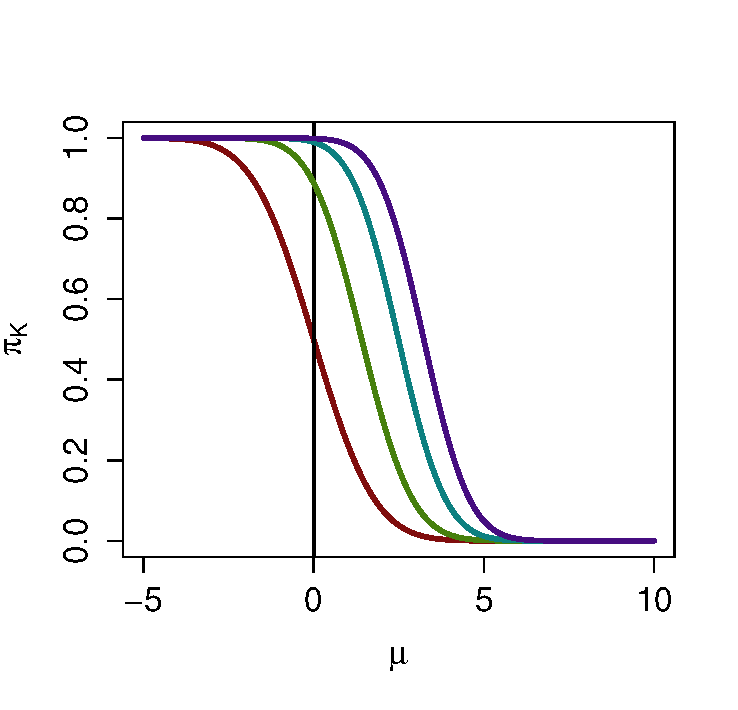
\includegraphics[scale = 0.5, clip=true, trim=0 0.2in 0 0.5in]{../info_theory_sims/illus_piK.pdf}
\caption{The function $pi_k(\mu)$, for $k = \{2, 9, 99, 999\}$ (left to right) \label{fig:pi}}
\end{figure}


First, let us rewrite $e_{ABE, k}$ in terms of the joint density $p(x, y)$.  Recall that the Bayes rule is
\[
e_{Bayes}(x_1,\hdots, x_k) = \frac{1}{k}\sum_{i=1}^k \Pr[\hat{X}(Y) \neq x_i| X = x_i].
\]
In turn, the Bayes classification rule is given in terms of the conditional density:
\[
\hat{X}(y) = \argmax_{x \in \{x_1,\hdots, x_k\}} p(y|x).
\]
Therefore, we obtain
\[
e_{Bayes}(x_1,\hdots, x_k) = \frac{1}{k}\sum_{i=1}^k \Pr[p(Y|x_i) \leq \max_{j \neq i} p(Y|x_j)| X = x_i].
\]
In turn the average Bayes error can be written as
\begin{align}
e_{ABE, k} &= \E[e_{Bayes}(X_1,\hdots, X_k)]
\\&= \frac{1}{k}\sum_{i=1}^k \E[\Pr[p(Y|x_i) \leq \max_{j \neq i} p(Y|x_j)| X = x_i]]
\\&= \E[\Pr[p(Y|x_1) \leq \max_{j \neq 1} p(Y|x_j)| X = x_1]]
\\&= \Pr[p(Y|X_1) \leq \max_{j \neq 1} p(Y|X_j)| X = X_1].
\end{align}

Defining $Z_i = \log p(Y|X_i) - \log p(Y|X_1)$, where $Y \sim p(y|X_1)$.
The we obtain
\[
e_{ABE} = \Pr[Z_1 < \max_{j > 1} Z_i].
\]

Our proof uses the assumption that $Z_1,\hdots, Z_k$ are asymptotically multivariate normal.
Supposing that $Z_1,\hdots, Z_k$ are indeed asymptotically normal, the following lemma
allows us to obtain a formula for the misclassification rate.

\textbf{Lemma 1. }
\emph{
Suppose $(Z_1, Z_2, \hdots, Z_k)$ are jointly multivariate normal, with 
$\E[Z_1 - Z_i]= \alpha$, 
$\Var(Z_1) = \beta$, 
$\Cov(Z_1, Z_i) = \gamma$, 
$\Var(Z_i)= \delta$, and $\Cov(Z_i, Z_j) = \epsilon$ for all $i, j = 2, \hdots,
k$, such that $\beta + \epsilon - 2\gamma > 0$.  Then, letting
\[
\mu = \frac{\E[Z_1 - Z_i]}{\sqrt{\frac{1}{2}\Var(Z_i - Z_j)}} = \frac{\alpha}{\sqrt{\delta - \epsilon}},
\]
\[
\nu^2 = \frac{\Cov(Z_1 -Z_i, Z_1 - Z_j)}{\frac{1}{2}\Var(Z_i - Z_j)} = \frac{\beta + \epsilon - 2\gamma}{\delta - \epsilon},
\]
we have
\begin{align*}
\Pr[Z_1 < \max_{i=2}^k Z_i] &= \Pr[W < M_{k-1}]
\\&= 1 - \int \frac{1}{\sqrt{2\pi\nu^2}} e^{-\frac{(w-\mu)^2}{2\nu^2}} \Phi(w)^{k-1} dw,
\end{align*}
where $W \sim N(\mu, \nu^2)$ and $M_{k-1}$ is the maximum of $k-1$
independent standard normal variates, which are independent of $W$.
}

\textbf{Proof.}
We can construct independent normal variates $G_1$, $G_2,\hdots, G_k$
such that
\[
G_1 \sim N(0, \beta + \epsilon - 2 \gamma)
\]
\[
G_i \sim N(0, \delta - \epsilon)\text{ for }i > 1
\]
such that
\[
Z_1 - Z_i = \alpha + G_1 + G_i \text{ for }i > 1.
\]
Hence
\begin{align*}
\Pr[Z_1 < \max_{i=2}^k Z_i] &= \Pr[\min_{i > 1} Z_1 - Z_i < 0].
\\&= \Pr[\min_{i=2}^{k} G_1 + G_i + \alpha < 0]
\\&= \Pr[\min_{i=2}^{k} G_i < -\alpha - G_1]
\\&= \Pr[\min_{i=2}^{k} \frac{G_i}{\sqrt{\delta - \epsilon}} < -\frac{\alpha - G_1}{\sqrt{\delta - \epsilon}}].
\end{align*}
Since $\frac{G_i}{\sqrt{\delta - \epsilon}}$ are iid standard normal variates, and since
$-\frac{\alpha - G_1}{\sqrt{\delta - \epsilon}} \sim N(\mu,\nu^2)$ for $\mu$ and $\nu^2$ given in the statement of the Lemma, the proof is completed via a straightforward computation.  $\Box$

To see why the assumption that $Z_1,\hdots, Z_k$ are multivariate normal might be justified, suppose that $X$ and $Y$ have the same dimensionality $d$, and that
joint density factorizes as
\[
p(x_j, y) = \prod_{i=1}^d p_i(x_{j, i}, y_i)
\]
where $x_{j, i}, y_i$ are the components of $x_j$ and $y$.
Then,
\[
Z_i = \sum_{m=1}^d \log p_m(y_m | x_{m, i}) - \log p_m(y_m | x_{m, 1})
\]
where $x_{i, j}$ is the $i$th component of $x_j$.
The $d$ terms $\log p_m(y_m | x_{m, i}) - \log p_m(y_m | x_{m, 1})$ are independent across the indices $m$,
but dependent between the $i = 1,\hdots, k$.
Therefore, the multivariate central limit theorem can be applied to conclude that the vector
$(Z_1,\hdots, Z_k)$ can be scaled to converge to a multivariate normal distribution.
Now, since the average Bayes error $e_{ABE,k}$ is a continuous functional of the joint distribution $p(x, y)$,
it follows that $e_{ABE,k}$ converges to a functional of the limiting mean and covariance of $(Z_1,\hdots, Z_k)$, assuming
that the limits exist.
In our theorem, we assume a specific regime where these limits exist as a consequence.
While the componentwise independence condition is not a realistic assumption,
the key property of multivariate normality of $(Z_1,\hdots, Z_k)$ holds under more general conditions, and appears reasonable in practice.

The second component of our theorem is to manipulate the expression of the mutual information $I(X; Y)$.
The differential mutual information is defined as
\[
I(X; Y) = \int p(x, y) \log \frac{p(x, y)}{p(x) p(y)} dx dy.
\]
The key manipulation we employ is to approximate the logarithmic term by the Taylor expansion
\[
\log \frac{p(x, y)}{p(x) p(y)} \approx \frac{p(x, y) - p(x) p(y)}{p(x) p(y)} - \left(\frac{p(x, y) - p(x) p(y)}{p(x) p(y)}\right)^2 + \hdots.
\]
The approximation is accurate if $I(X; Y)$ is small--or rather, small relative to the dimensionality within the asymptotic sequence.
We state the theorem for the regime where $I(X; Y)$ is fixed, while the dimensionality of $X$ increases.

\subsection{Technical section}

We formally state the assumptions and theorem in this section.  The
less technically inclined reader may skip the section in order to
continue to the proposed methodology for estimating mutual
information, and results.

The asymptotic regime we consider is one where the dimension of $X$ goes to infinity.
This means that we have to consider a sequence of joint distributions $(X^{[d]}, Y^{[d]})$ indexed by the dimension $d$.

Fix integer $k \geq 2$.  Let $p^{[d]}(x,y)$ be a sequence of
probability density functions, where $x$ is of dimension $p^{[d]}$ and
$y$ is of dimension $q^{[d]}$.  Let $p^{[d]}(x)$ and $p^{[d]}(y)$
denote the marginal densities, and let
\[
p^{[d]}(y|x) = p^{[d]}(x, y)/p^{[d]}(y).\]
 Let $(X^{([d], i)}, Y^{([d], i)})$ be
iid random variates from $p^{[d]}(x, y)$ for $i = 1, \hdots, k$; we will supress the
superscripts $[d]$ and/or $(i)$ when convenient.  Recall the definitions of
entropy,
\[
H(X) = -\int p(x) \log p(x) dx,
\]
and mutual information
\[
I(X; Y) = \int p(x, y) \log \frac{p(x, y)}{p(x)p(y)} dx dy.
\]
Furthermore, define the $K$-class average Bayes error as
\[
e_{ABE, k} = \Pr[p(Y^{(1)}|X^{(1)}) < \max_{i = 2}^{k} p(Y^{(1)}|X^{(i)})].
\]
Define
\[
u^{[d]}(x, y) = \log p^{[d]}(x, y) - \log p^{[d]}(x) - \log p^{[d]}(y),
\]
and define
\[
\ell_{ij}^{[d]} = \log p(y^{(i)}|x^{(j)}).
\]



We now give the theorem and its proof.

\textbf{Theorem 1.} Let $p^{[d]}(x, y)$ be a sequence of joint densities
for $d = 1,2,\hdots$ as given above.  Further assume that
\begin{itemize}
\item[A1.] $\lim_{d \to \infty} I(X^{[d]}; Y^{[d]}) = \iota < \infty.$
\item[A2.] There exists a sequence of scaling constants $a_{ij}^{[d]}$
and $b_{ij}^{[d]}$ such that the random vector $(a_{ij}\ell_{ij}^{[d]} +
b_{ij}^{[d]})_{i, j = 1,\hdots, k}$ converges in distribution to a
multivariate normal distribution.
\item[A3.] There exists a sequence of scaling constants $a^{[d]}$, $b^{[d]}$ such that
\[
a^{[d]}u(X^{(1)}, Y^{(2)}) + b^{[d]}
\]
converges in distribution to a univariate normal distribution.
\item[A4.] For all $i \neq k$,
\[\lim_{d \to \infty}\Cov[u(X^{(i)}, Y^{(j)}), u(X^{(k)}, Y^{(j)})] = 0.\]
\end{itemize}
Then for $e_{ABE, k}$ as defined above, we have
\[
\lim_{d \to \infty} e_{ABE, k} = \pi_k(\sqrt{2 \iota})
\]
where
\[
\pi_k(c) = 1 - \int_{\mathbb{R}} \phi(z - c)  \Phi(z)^{k-1} dz
\]
where $\phi$ and $\Phi$ are the standard normal density function and
cumulative distribution function, respectively.

%[[Maybe add remark about assumptions here.]]

\textbf{Proof.}

For $i = 2,\hdots, k$, define
\[
Z_i = \log p(Y^{(1)}|X^{(i)}) - \log p(Y^{(1)}|X^{(1)}).
\]
Then, we claim that $\vec{Z} = (Z_2,\hdots, Z_k)$ converges in distribution to
\[
\vec{Z} \sim N\left(-2\iota, 
\begin{bmatrix}
4\iota & 2\iota & \cdots & 2\iota\\
2\iota & 4\iota & \cdots & 2\iota\\
\vdots & \vdots & \ddots & \vdots\\
2\iota & 2\iota & \cdots & 4\iota
\end{bmatrix}
\right).
\]
Combining the claim with the lemma (stated below this proof) yields the
desired result.

To prove the claim, it suffices to derive the limiting moments
\[\E[Z_i] \to -2\iota,\]
\[\Var[Z_i] \to 4\iota,\]
\[\Cov[Z_i, Z_j] \to 2\iota,\]
for $i \neq j$,
since then assumption A2 implies the existence of a multivariate normal
limiting distribution with the given moments.

Before deriving the limiting moments, note the following identities.
Let $X' = X^{(2)}$ and $Y = Y^{(1)}$.
\[
\E[e^{u(X', Y)}] = \int p(x) p(y) e^{u(x, y)} dx dy = \int p(x, y) dx dy = 1.
\]
Therefore, from assumption A3 and the formula for gaussian exponential
moments, we have
\[
\lim_{d \to \infty} \E[u(X', Y)]-\frac{1}{2}\Var[u(X', Y)] = 0.
\]
Let $\sigma^2 = \lim_{d \to \infty} \Var[u(X', Y)]$.
Meanwhile, by applying assumption A2,
\begin{align*}
\lim_{d \to \infty} I(X; Y) &= \lim_{d \to \infty} \int p(x, y) u(x, y) dx dy 
= \lim_{d \to \infty} \int p(x) p(y) e^{u(x, y)} u(x, y) dx dy
\\&= \lim_{d \to \infty}  \E[e^{u(X, Y')}u(X, Y')]
\\&= \int_{\mathbb{R}} e^z z \frac{1}{\sqrt{2\pi \sigma^2}} 
e^{-\frac{(z + \sigma^2/2)^2}{2\sigma^2}} \text{ (applying A2)}
\\&= \int_{\mathbb{R}} z \frac{1}{\sqrt{2\pi \sigma^2}} 
e^{-\frac{(z - \sigma^2/2)^2}{2\sigma^2}}
\\&= \frac{1}{2}\sigma^2.
\end{align*}
Therefore,
\[
\sigma^2 = 2\iota,
\]
and
\[
\lim_{d \to \infty} \E[u(X', Y)] = -\iota.
\]
Once again by applying A2, we get
\begin{align*}
\lim_{d \to \infty} \Var[u(X, Y)] 
&= \lim_{d \to \infty} \int (u(x, y) - \iota)^2 p(x, y) dx dy
\\&= \lim_{d \to \infty} \int (u(x, y) - \iota)^2 e^{u(x, y)} p(x) p(y) dx dy
\\&= \lim_{d \to \infty} \E[(u(X', Y) - \iota)^2 e^{u(X', Y)}] 
\\&= \int (z - \iota)^2 e^z \frac{1}{\sqrt{4\pi\iota}} e^{-\frac{(z+\iota)^2}{4\iota}} dz \text{ (applying A2)}
\\&= \int (z - \iota)^2 \frac{1}{\sqrt{4\pi\iota}} e^{-\frac{(z-\iota)^2}{4\iota}} dz
\\&= 2\iota.
\end{align*}


We now proceed to derive the limiting moments.
We have
\begin{align*}
\lim_{d \to \infty} \E[Z] 
&= \lim_{d \to \infty} \E[ \log p(Y|X') - \log p(Y|X)]
\\&= \lim_{d \to \infty} \E[ u(X', Y) - u(X, Y) ] = -2\iota.
\end{align*}
Also,
\begin{align*}
\lim_{d \to \infty} \Var[Z]
 &= \lim_{d \to \infty} \Var[ u(X', Y) - u(X, Y) ]
\\&= \lim_{d \to \infty} \Var[ u(X', Y)] +\Var[ u(X, Y) ]\text{ (using assumption A4) }
\\&= 4\iota,
\end{align*}
and similarly
\begin{align*}
\lim_{d \to \infty} \Cov[Z_i, Z_j]
&= \lim_{d \to \infty} \Var[ u(X, Y)]\text{ (using assumption A4) }
\\&= 2\iota.
\end{align*}
This concludes the proof. $\Box$.

Assumptions A1-A4 are satisfied in a variety of natural models.
One example is a multivariate Gaussian model where
\[
X \sim N(0, \Sigma_d)
\]
\[
E \sim N(0, \Sigma_e)
\]
\[
Y = X + E
\]
where $\Sigma_d$ and $\Sigma_e$ are $d \times d$ covariance matrices, and where $X$ and $E$ are independent.  Then, if $d \Sigma_d$ and $\Sigma_e$ have limiting spectra $H$ and $G$ respectively,
the joint densities $p(x, y)$ for $d = 1,\hdots, $ satisfy assumptions A1 - A4.

We can also construct a family of densities satisfying A1 - A4,
which we call an \emph{exponential family sequence model} since each joint distribution in the sequence
is a member of an exponential family.
A given exponential family sequence model is specified by choice of a base carrier function $b(x, y)$ and base sufficient statistic $t(x, y)$, with the property that carrier function factorizes as
\[
b(x, y) = b_x(x) b_y(y)
\]
for marginal densities $b_x$ and $b_y$.
Note that the dimensions of $x$ and $y$ in the base carrier function are arbitrary;
let $p$ denote the dimension of $x$ and $q$ the dimension of $y$ for the base carrier function.
Next, one specifies a sequence of scalar parameters $\kappa_1, \kappa_2,\hdots$ such that
\[
\lim_{d \to \infty} d \kappa_d = c < \infty.
\]
for some constant $c$.
For the $d$th element of the sequence, $X^{[d]}$ is a $pd$-dimensional vector,
which can be partitioned into blocks
\[
X^{[d]} = (X_1^{[d]},\hdots, X_d^{[d]})
\]
where each $X_i^{[d]}$ is $p$-dimensional.  Similarly, $Y^{[d]}$ is partitioned into $Y_i^{[d]}$ for $i = 1,\hdots, d$.
The density of $(X^{[d]}, Y^{[d]})$ is given by
\[
p^{[d]}(x^{[d]}, y^{[d]}) = Z_d^{-1} \left(\prod_{i=1}^d b(x_i^{[d]}, y_i^{[d]}) \right) 
\exp\left[\kappa_d \sum_{i=1}^d t(x_i^{[d]}, y_i^{[d]}) \right],
\]
where $Z_d$ is a normalizing constant.
Hence $p^{[d]}$ can be recognized as the member of an exponential family with carrier measure
\[
\left(\prod_{i=1}^d b(x_i^{[d]}, y_i^{[d]}) \right)
\]
and sufficient statistic
\[
\sum_{i=1}^d t(x_i^{[d]}, y_i^{[d]}).
\]

One example of such an exponential family sequence model is a
multivariate Gaussian model with limiting spectra $H = \delta_1$ and
$G = \delta_1$, but scaled so that the marginal variance of the
components of $X$ and $Y$ are equal to one.  This corresponds to a
exponential family sequence model with
\[
b_x(x) = b_y(x) = \frac{1}{\sqrt{2\pi}} e^{-x^2/2}
\]
and
\[t(x, y) = xy.\]

Another example is a multivariate logistic regression model,
given by
\[
X \sim N(0, I)
\]
\[
Y_i \sim \text{Bernoulli}(e^{\beta X_i}/(1 + e^{\beta X_i}))
\]
This corresponds to an exponential family sequence model with
\[
b_x(x) = \frac{1}{\sqrt{2\pi}} e^{-x^2/2}
\]
\[
b_y(y) = \frac{1}{2}\text{ for }y = \{0, 1\},
\]
and
\[
t(x, y) = x\delta_1(y) - x\delta_0(y).
\]
The multivariate logistic regression model (and multivariate Poisson regression model)
are especially suitable for modeling neural spike count data;
we simulate data from such a multivariate logistic regression model in section X.

\subsection{Inference for mutual information}

In the previous section, we showed that
\[
\lim_{d \to \infty} e_{ABE, k} = \pi_k(\sqrt{2 I(X; Y)}),
\]
where $e_{ABE, k}$ is the $k$-class average Bayes error,
in an asymptotic regime where $I(X^{[d]}; Y^{[d]})$ is fixed while the dimensionality of $X$ increases.
Since $\pi_k$ is invertible for all $k = 2, \hdots$,
a converse relationship
\[
\lim_{d \to \infty} I(X^{[d]}; Y^{[d]}) = \frac{1}{2}(\pi_k^{-1}(\eta))^2
\]
also holds in the same regime.  We formally state the result, and a few consequences, as follows.

\textbf{Corollary 1.}
Let $p^{[d]}(x, y)$ be a sequence of joint densities
for $d = 1,2,\hdots$ as given above.  Further assume assumptions A2 - A4 and also
\begin{itemize}
\item[A1'.] $\lim_{d \to \infty} e_{ABE, k} = \eta < \infty.$
\end{itemize}
Then
\begin{itemize}
\item[i.]
\[
\lim_{d \to \infty} I(X^{[d]}; Y^{[d]}) = \frac{1}{2}(\pi_k^{-1}(e_{ABE}))^2.
\]
\item[ii.]
If $[\underline{e}, \bar{e}]$ is a $1-\alpha$ confidence interval for $e_{ABE, k}$,
then
\[
[\frac{1}{2}(\pi_k^{-1}(\bar{e}))^2, \frac{1}{2}(\pi_k^{-1}(\underline{e}))^2]
\]
is asymptotically a $1-\alpha$ confidence interval of $I(X; Y)$: that is,
\[
\lim_{d \to \infty} \Pr\left[I(X^{[d]}; Y^{[d]}) \in [\frac{1}{2}(\pi_k^{-1}(\underline{e}))^2, \frac{1}{2}(\pi_k^{-1}(\bar{e}))^2]\right] = 1-\alpha.
\]
\item[iii.] If $\hat{e}$ is a $O(1/\sqrt{n})$-consistent estimator for $e_{ABE, k}$,
and $\lim_{d \to \infty} e_{ABE, k} > 0,$
then $\frac{1}{2}(\pi_k^{-1}(\hat{e}))^2$ is a $O(1/\sqrt{n})$-consistent estimator for $I(X; Y)$.
\end{itemize}

\textbf{Proof.} 

(i) Let $\{\iota_1,\hdots, \}$ be a collection of limiting points of $I(X^{[d]}; Y^{[d]})$.
By Theorem 1, each of the corresponding subsequences has $e_{ABE, k}$ converging to
$\pi_k(\sqrt{2 \iota_i})$.  However, by assumption A1', $e_{ABE, k}$ converges to $\eta$ in
all subsequences.  Therefore, 
\[\iota_1 = \iota_2 = \cdots = \frac{1}{2}(\pi_k^{-1}(\eta))^2,\]
implying the corollary.

The proof of (ii) follows from continuity of probability, while the proof of (iii) follows from application of the delta method.  $\Box$

As corollary 1 states, it is possible to construct a confidence interval for $I(X; Y)$ by
first constructing a confidence interval for the average Bayes error $e_{ABE,
k}$; then obtaining the confidence interval for $I(X; Y)$ as
\[
[\frac{1}{2}(\pi_k^{-1}(\bar{e}))^2, \frac{1}{2}(\pi_k^{-1}(\underline{e}))^2].
\]

Corollary 1 also gives the consisistent point estimate
\[\hat{I}(X; Y) = \frac{1}{2}(\pi_k^{-1}(\hat{e}))^2,\]
where $\hat{e}$ is a $O(1/\sqrt{n})$-consistent estimate of $e_{ABE,
k}.$ However, $\hat{I}(X, Y)$ may perform poorly in finite samples due
to bias.  Better performance can be obtained by using bias-correction
and shrinkage, but the optimality of the estimator depends on the
choice of risk function and risk criterion.  In the remainder
of the paper, we will be mainly interested in interval estimation.


%However, this procedure for obtaining point estimates can be easily seen to have suboptimal mean-squared risk in finite samples.
%Suppose that the estimator for average Bayes error has bias
%\[
%\E[\hat{e}] - e_{ABC, k} = \mu
%\]
%and variance
%\[
%\Var[\hat{e}] = \sigma^2,
%\]
%and assume that $\mu$ is $O(1/\sqrt{n})$ while $\sigma^2$ is $O(1/n)$.
%Let $f(e) = \frac{1}{2}(\pi_k^{-1}(e))^2$.
%We know that
%\[
%\lim_{e \to 0} f(e) = \infty,
%\]
%and also that
%\[
%\lim_{e \to 0} f'(e) = -\infty,
%\]
%\[
%\lim_{e \to 0} f''(e) = \infty.
%\]
%Meanwhile, from the delta method we have
%\[
%\E[\hat{I}] = \E[f(\hat{e})] = I(X; Y) + \mu f'(e_{ABC, k}) + \frac{1}{2} \sigma^2 f''(e_{ABC, k}),
%\]
%and
%\[
%\Var[\hat{I}] = \hdots.
%\]
%[to be continued.  Task: propose a better estimator in mean-squared error.]

\section{Applications}

Having established the theoretical basis of our method, the current
section is dedicated to discussing applications and practical issues.
In contrast to the previous section, our focus in this section will be
methodological rather than theoretical.

Within the framework of randomized designs, a number of
machine-learning-based modeling approaches can be applied to assess
informativity.  The most common approaches are based
on \emph{classification} and \emph{regression}, but a third
approach, \emph{identification}, combines the strengths of both
classification and regression.

The different machine-learning-based modeling approaches excel in
different experimental settings.  Classification-based approaches
require large amounts of training data and test data for a small
number of stimuli categories.  Therefore, an investigator intending to
use classification will design the experiment to have a large number
of repeats relative to the number of stimulus categories.

In contrast, in the identification-based approach, it is not necessary
to have multiple repeats for each stimulus exemplar.  On the other
hand, it \emph{is} necessary to have a parameterization of the
stimulus exemplars.  The success of the identification approach
depends heavily on having a parameterization which captures the
relevant features of the stimulus--this can be a difficult task when
studying complex stimuli such as faces or natural images.

While we described the classification
approach in section 2, we describe the application of our method using
classifiers in section 4.1.  Then, in section 4.2, we will introduce
the identification task, and how our method can also be combined with
the identification-based approach.


\subsection{Classification setting}

Recall the notation used in section 2.1: the $k$ stimuli exemplars are
denoted $\{x^{(1)},\hdots, x^{(k)}\}$ and the $r$ responses for the
$i$th class are given by $y^{(i), 1},\hdots, y^{(i), r}$.

For a given classifier $\mathcal{F}$, the classification rule $f$ varies randomly depending on the input.
One can define the average generalization error
\[
e_{AGE} = \E[e_{gen}(\mathcal{F}(\{(x^{(1)}, Y^{(1),1}),\hdots, (x^{(1)},Y^{(1),r_1}), \hdots, (x^{(k)}, Y^{(k),1},\hdots, (x^{(k)},Y^{(k), r_1})\}))]
\]
where the expectation is taken over the sampling of the training
data \emph{conditional} on fixing the stimuli $x^{(1)},\hdots,
x^{(r)}.$ The procedure we suggest for obtaining a confidence interval
for $\hat{I}(X; Y)$ is to first obtain a confidence interval for the
average generalization error, $[\underline{e}, \bar{e}]$, then apply
the inversion formula to construct the interval\footnote{Note that the theory established in section 3.2 does not apply to the
coverage properties of $C$, since we used a confidence interval for
$e_{AGE}$ rather than $e_{Bayes}$ to construct the interval.  Despite
this limitation, the resulting interval $C$ still serves the useful
purpose of conveying the uncertainty about the inferred information.}
\[
C = [\frac{1}{2}(\pi_k^{-1}(\bar{e}))^2, \frac{1}{2}(\pi_k^{-1}(\underline{e}))^2].
\]

We can use cross-validation to construct such a confidence interval
$C$.  For a large number of resampling trials $B$, let $S_1,\hdots,
S_B$ be random subsets of the data such that each $S_i$ consists of
$r_1$ repeats for each stimulus\footnote{ That is, let $\rho^{i,
j}(\ell)$ be a random injective mapping from $\{1,\hdots, r_1\}$ to
$\{1,\hdots, r\}$ for each $i = 1,\hdots, B$ and $j = 1,\hdots, k$.
The $\rho^{i,j}$ are i.i.d. from the uniform distribution on such
mappings.  Define $S_i = \{(x^{(j)}, y^{(j), \rho^{i, j}(\ell)})|
1 \leq \ell\leq r \text{ and }1\leq j \leq k\}$. Meanwhile, define
$\bar{S}_i = \{(x^{(j)}, y^{(j), \ell})|1\leq j\leq k, 1\leq \ell \leq
r\}\setminus S_i$. }.  Let $\bar{S}_i$ denote the complement of $S_i$
in the data.  For each $i = 1,\hdots, B$, construct a classification
rule $f^{(i)}$ by inputting the set $S_i$ as training data for the
classifier,
\[
f^{(i)} = \mathcal{F}(\{(x, y): (x, y) \in S_i\})
\]
Define the $i$th estimate of test error
as
\[
e^{(i)} = \frac{1}{kr_2} \sum_{j=1}^{k}\sum_{(x^{(j)}, y) \in \bar{S}_i} I(f(y) \neq j).
\]

In both cases, the general idea is to first assume that the
generalization error $e_{AGE}$ of the classifer $\mathcal{F}$
approximates the Bayes error


\subsection{Identification setting}


\section{Results}

\subsection{Simulation}

Multiple-response logistic regression model
\[
X \sim N(0, I_p)
\]
\[
Y \in \{0,1\}^q
\]
\[
Y_i|X = x \sim \text{Bernoulli}(x^T B_i)
\]
where $B$ is a $p \times q$ matrix.

\emph{Methods.}
\begin{itemize}
\item \text{Nonparametric}: $\hat{I}_0$ naive estimator, $\hat{I}_\alpha$ anthropic correction.
\item \text{ML-based}: $\hat{I}_{CM}$ confusion matrix, $\hat{I}_F$ Fano, $\hat{I}_{LS}$ low-SNR method.
\end{itemize}

Sampling distribution of $\hat{I}$ for \small{$\{p = 3$, $B = \frac{4}{\sqrt{3}} I_3$, $K = 20$, $r = 40\}$.}

True parameter $I(X; Y) = 0.800$ \emph{(dotted line.)}
\begin{center}
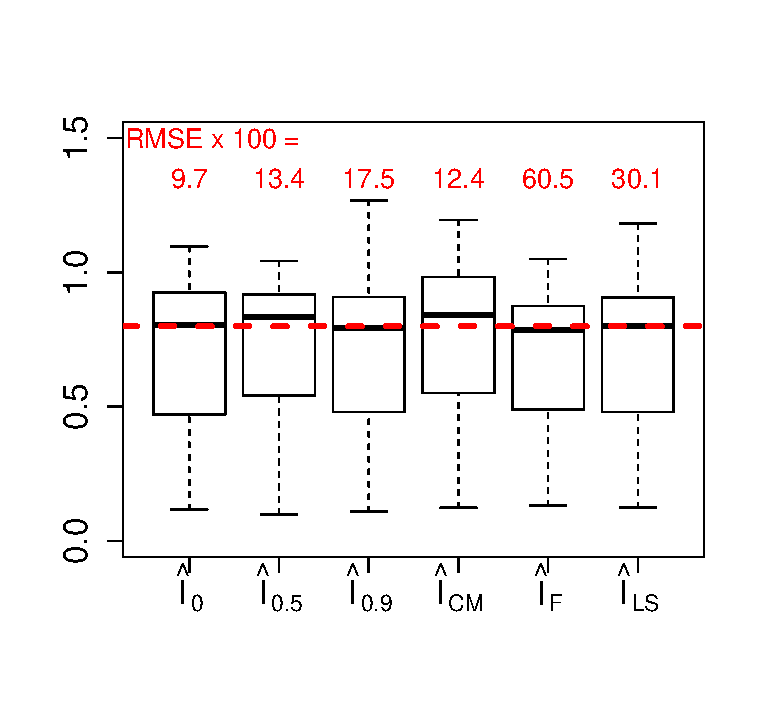
\includegraphics[scale = 0.5, clip = true, trim = 0 0.5in 0 0.5in]{../info_theory_sims/fig1.pdf}
\end{center}
Na\"{i}ve estimator performs best!  $\hat{I}_{LS}$ not effective.

Sampling distribution of $\hat{I}$ for \small{$\{p = 50$, $B = \frac{4}{\sqrt{50}} I_{50}$, $K = 20$, $r = 8000\}$.}

True parameter $I(X; Y) = 1.794$ \emph{(dashed line.)}
\begin{center}
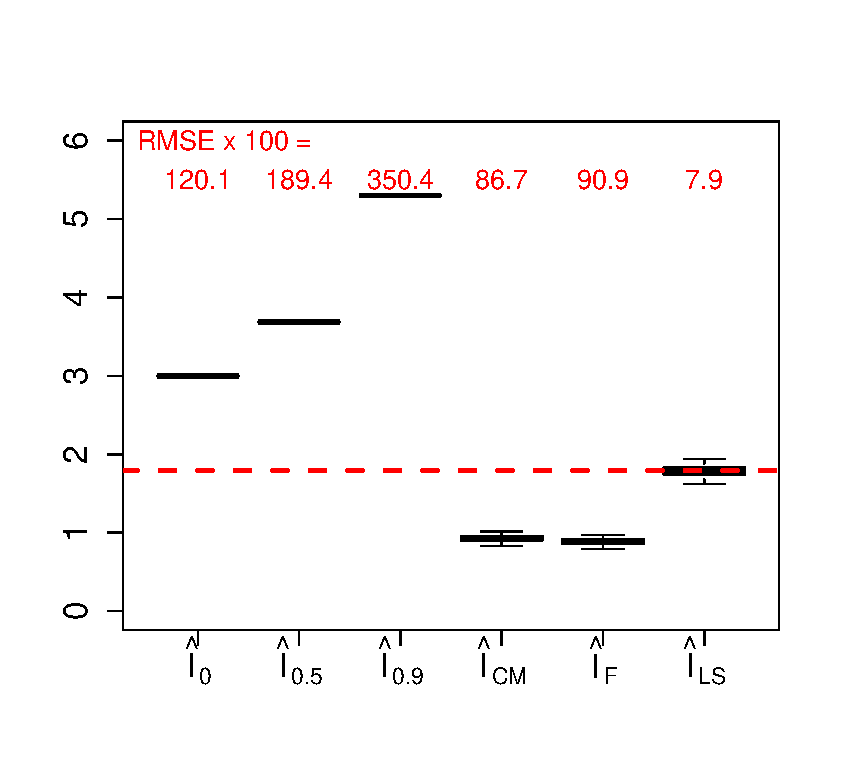
\includegraphics[scale = 0.5, clip = true, trim = 0 0.5in 0 0.5in]{../info_theory_sims/fig2.pdf}
\end{center}
Non-parametric methods extremely biased.

Estimation path of $\hat{I}_{LS}$ and $\hat{I}_\alpha$ as $n$ ranges from $10$ to $8000$.

\small{$\{p = 10$, $B = \frac{4}{\sqrt{10}} I_{10}$, $K = 20\}$.
True parameter $I(X; Y) = 1.322$ \emph{(dashed line.)}}

\begin{center}
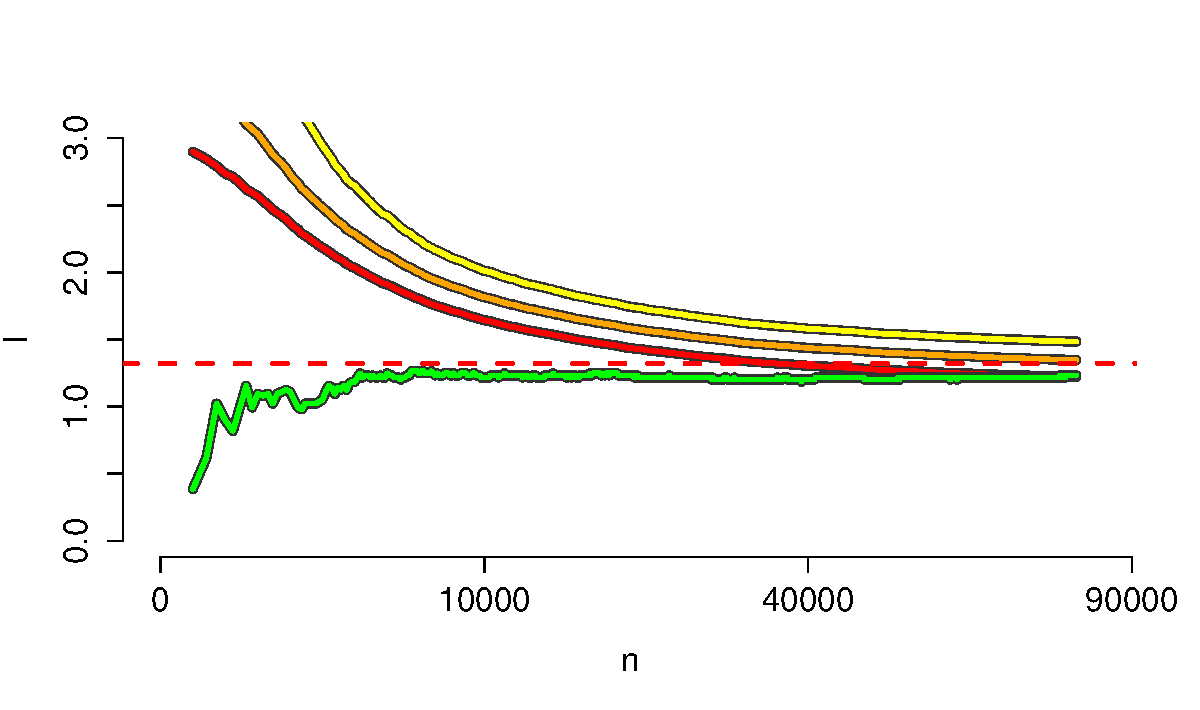
\includegraphics[scale = 0.4]{../info_theory_sims/fig3.pdf}
\end{center}

\begin{center}
\textbf{Estimated $\hat{I}$ vs true $I$.} 

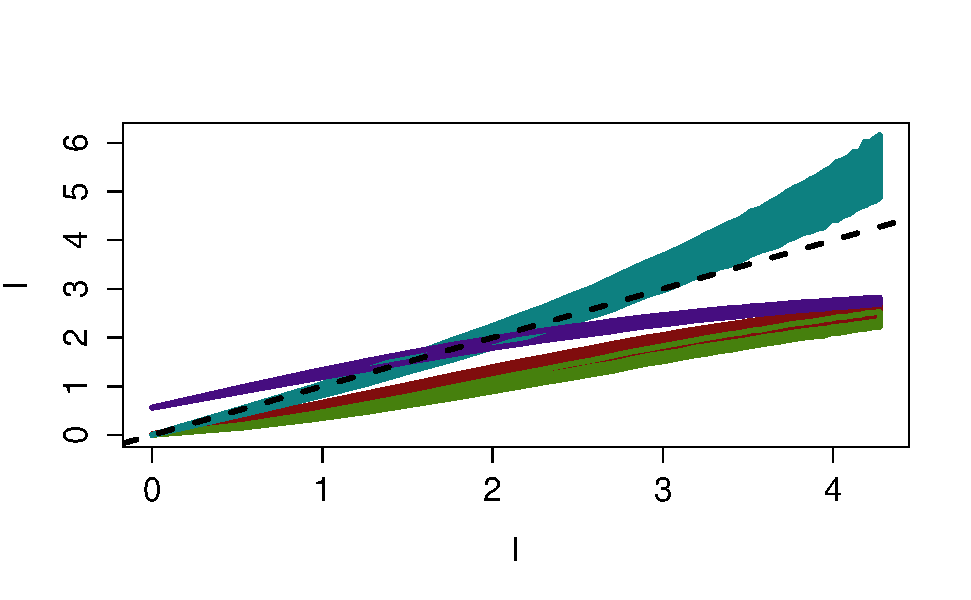
\includegraphics[scale = 0.5, clip=true, trim=0.4in 0.5in 0 0.5in]{../info_theory_sims/fig4.pdf}
\end{center}

Sampling distribution of $\hat{I}_{LS}$ for \small{$\{p = 10$, $B = \frac{4}{\sqrt{10}} I_{10}$, $N = 80000\}$,

and $K = \{5, 10, 15, 20, \hdots, 80\}$, $r = N/k$.}

True parameter $I(X; Y) = 1.322$ \emph{(dashed line.)}
\begin{center}
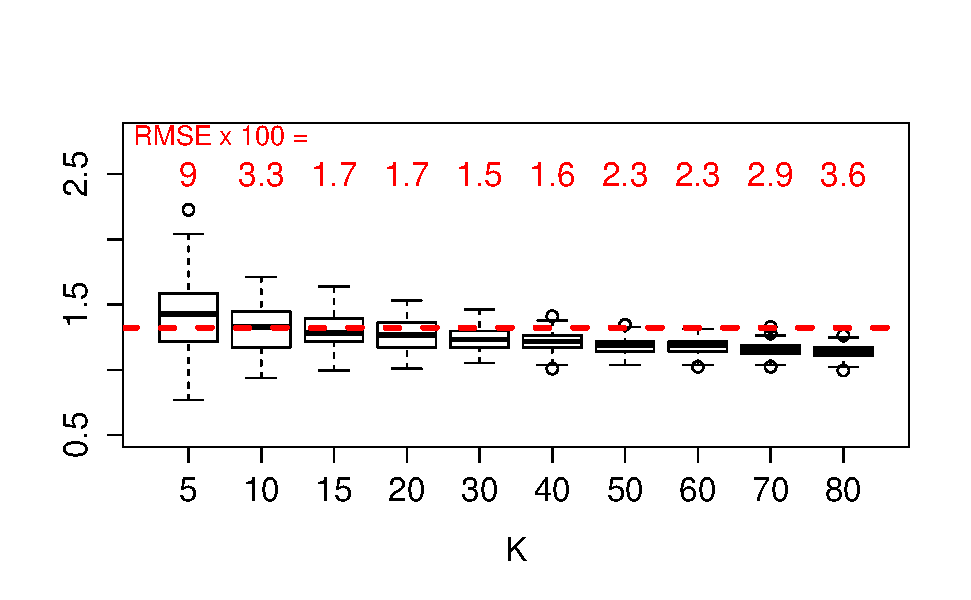
\includegraphics[scale = 0.6, clip = true, trim = 0 0.5in 0 0.5in]{../info_theory_sims/fig5a.pdf}
\end{center}

Decreasing variance as $K$ increases. Bias at large and small $K$.

$p = 20$ and $q = 40$, entries of $B$ are iid $N(0, 0.025)$.

$K=20$, $r = 8000$, true $I(X; Y) = 1.86$ \emph{(dashed line.)}

\begin{center}
\textbf{Sampling distribution of $\hat{I}$.}
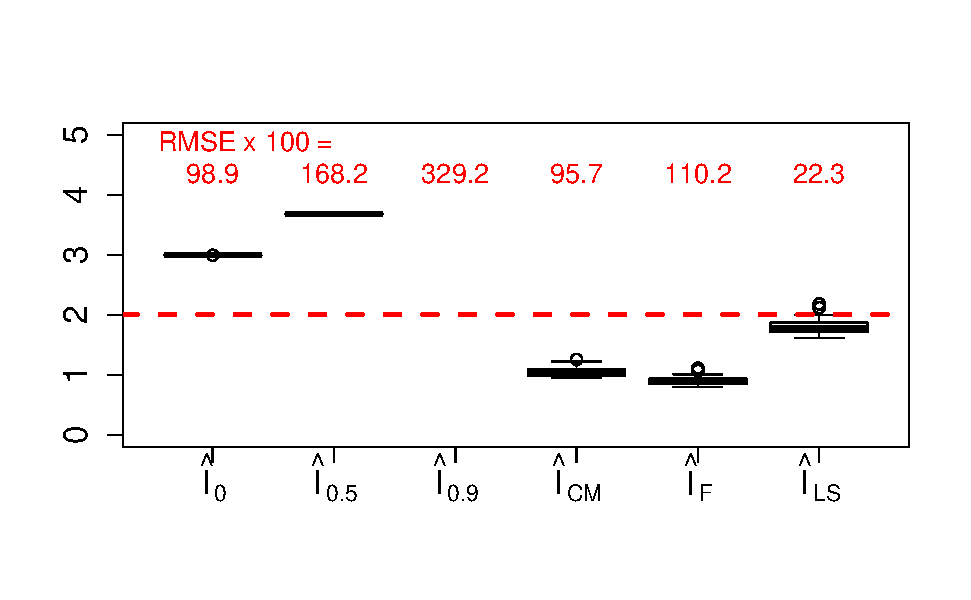
\includegraphics[scale = 0.6, clip = true, trim = 0 0.5in 0 0.5in]{../info_theory_sims/fig6.pdf}
\end{center}

\subsection{Application to data}

Kay et al. employed a randomized stimuli design in their 2008 paper,
``Identifying Natural Images from Human Brain Activity.''  The
experiment was designed in order to investigate how visual information
from natural images is encoded in the V1 through V3 brain regions.
The stimulus space, $\mathcal{X}$, consists of $128 \times 128$-pixel
grayscale photographs.  The response data consists of BOLD response in
regions V1, V2, and V3 from a single subject.  The raw time series were
processed to yield a single averaged response vector $y^{(i)}$ for each
stimulus $x^{(i)}$, for $i = 1,\hdots, 1870$.
The dimensionality of $y^{(i)}$ varies depending on which regions of interest
we are discussing, and whether we consider a subset of the voxels in those regions.
Let $v$ denote the dimensionality (number of voxels) of $y$.

Let $x^{(i)}$ denote the native $128 \times 128$-pixel representation
of the image (i.e. a $16384$-dimensional vector with entries between 0
and 1.)  One of the goals of the Kay et al. paper is to evaluate
competing encoding models.  In the context of the study,
an \emph{encoding model} is a vector-valued function from the stimulus
to a $p$-dimensional space,
\[
\vec{g}(x) = (g_1(x),\hdots, g_{p}(x)).
\]
One of the encoding models studied by Kay et al. is the Gabor wavelet pyramid,
$\vec{g}_{Gabor}$, with $p = 10921$.
Using a \emph{training} subset of the stimulus-response pairs $(x_i, y_i)$, $i = 1,\hdots, 1750$,
Kay et al. fit a regularized linear model
\[
y^{(i)} \approx B^T \vec{g}(x^{(i)})
\]
where $B$ is a $10921 \times v$-dimensional matrix, which is to be fit to the data.
The resulting model is used to obtain predictions $\hat{y}^{(i)}$ for the remaining validation subset,
$i = 1751,\hdots, 1870$,
by
\[
\hat{y}^{(i)} = B^T \vec{g}(x^{(i)}).
\]
Kay et al. introduced the novel idea of assessing the accuracy of
these predictions using a \emph{classification}-based metric, rather
than a usual metric for prediction error such as mean-squared error.
One treats the 120 validation stimuli $x_{1751},\hdots, x_{1870}$ as distinct classes.
Next, for each $i = 1751, \hdots, 1870$, one predicts the class of $y^{(i)}$,
by correlating the observed $y^{(i)}$ with the predictions $\hat{y}^{(j)}$.
In other words, let $f$ be the mapping from the observed response to the predicted class:
$f$ is given by
\[
f(y) = \argmax_{j =1751}^{1870} \Cor(y, \hat{y}^{(j)}).
\]
The test error is
\[
e_{test} = \frac{1}{120} \sum_{i=1751}^{1870} I(i \neq f(y^{(i)})).
\]
This test error can be computed using different encoding models
$\vec{g}$ and different regions of the brain, or different-sized
subsets of voxels.
One can therefore get a sense of the differences between encoding models
or between brain regions by comparing the resulting test errors.


While differing from a conventional classification task, the Kay et
al. \emph{identification} task can also be treated using our
framework.  An \emph{identification rule} (as opposed to a
classification rule) is defined by a function $f$ which takes arguments
$\{y, x^{(1)},\hdots, x^{(k)}\}$ where $k$ can be any positive integer.
The function $f$ returns an integer from 1 to $k$,
\[
f(y, x^{(1)},\hdots, x^{(k)}) \in \{1,\hdots, k\}.
\]
One can study competing encoding models by constraining identification rules
to using features provided by the encoding, i.e. only considering functions
\[
f(y, \vec{g}(x^{(1)}),\hdots, \vec{g}(x^{(k)})) \in \{1,\hdots, k\}.
\]

The generalization error for the identification task is defined as
\[
e_{gen}(f) = \Pr[f(Y, \vec{g}(x^{(1)}),\hdots, \vec{g}(x^{(k)})) \neq i|Y \sim p(y|x^{(i)})],
\]
Now, the Bayes rule will be specific to the encoding model
\[
e_{Bayes}(\vec{g}(x^{(1)}),\hdots, \vec{g}(x^{(k)})) = \inf_f \Pr[f(Y, \vec{g}(x^{(1)}),\hdots, \vec{g}(x^{(k)})) \neq i|Y \sim p(y|x^{(i)})].
\]
As before, the Bayes identification rule which attains the minimal error can be given explicitly,
\[
f_{Bayes}(y, \vec{g}(x^{(1)}),\hdots, \vec{g}(x^{(k)})) = \argmin_{i=1}^k p(y|\vec{g}(x^{(i)})).
\]
The average Bayes error can be defined as before, but is specific to the encoding model:
\[
e_{ABE}(\vec{g}) = \E[e_{Bayes}(\vec{g}(X^{(1)}),\hdots, \vec{g}(X^{(k)}))]
\]

Our asymptotic theory links average Bayes error to information and
is \emph{not specific} to the whether the task is based on
identification or classification.  Hence, the approximation
\[
e_{ABE, k}(\vec{g}) \approx \pi_k(\sqrt{2 I(\vec{g}(X); Y)})
\]
still holds in the appropriate regime.


However, one adjustment that needs to be made is how to construct
point estimates or confidence intervals for $e_{ABE}$.
Here we will limit our discussion to confidence intervals.
The approach taken is to use cross-validation to construct the confidence interval.

Let $N$ be the total number of stimuli exemplars.  Choose $T < N$ and
$k < N - T$; $T$ denotes the number of \emph{training} exemplars and
$k$ controls the number of \emph{test} exemplars.

Set $B$, the number of Monte Carlo simulations, to be a large number.
Let $\beta \in [0, 1]$ be a Bayesian smoothing parameter (typically $\beta$ is close to 0).
For each $b = 1,\hdots, B$, define the $b$th sampled test error $e_b$ by:
\begin{enumerate}
\item Sample $T$ stimuli exemplars without replacement from the library of $N$ exemplars.
\item Train an identification rule $f_b$ using the training set pairs $(\vec{g}(x^{(i)}), y^{(i)})$.
\item Let $S_1,\hdots, S_M$ denote all possible subsets of size $k$ from the remaining $N-T$ exemplars.
\item For each subset $S_j = \{x^{(i_{j, 1})}, \hdots, x^{(i_{j, k})}\}$, compute the test error $e_{test, b, j}$ via
\[
e_{test, b, j} = \frac{1}{k} \sum_{\ell = 1}^k I(i_{j, \ell} \neq f(y^{(i_{j, \ell})}, \vec{g}(x^{(i_{j, 1})}),\hdots, \vec{g}(x^{(i_{j, k})})))
\]
\item Set $e_b = \beta\frac{k-1}{k} + (1-\beta) \frac{1}{M} \sum_{j=1}^M e_{test, b, j}$.
\end{enumerate}
For most identification rules, $e_b$ can be computed in $O(N^2)$ time
by using the hypergeometric sampling formula; e.g., see Nishimoto
(2011) for details.  Setting the parameter $\beta > 0$ is typically
recommended in order to reduce variance in the procedure.

Now, choosing a level $\alpha$, let $\bar{e}(\vec{g})$ be the $(1-\alpha/2)$th
quantile and $\underline{e}(\vec{g})$ be the $(\alpha/2)$th quantile of
$\{e_b\}_{b=1}^B$.  Then one constructs the confidence interval
\[
[\frac{1}{2}(\pi_k^{-1}(\bar{e}))^2, \frac{1}{2}(\pi_k^{-1}(\underline{e}))^2].
\]
for $I(\vec{g}(X); Y)$.

We computed such confidence intervals for $\vec{g}_{Gabor}$, taking
$Y$ to be random subsamples of size $\{100, 200, \hdots, 600\}$ voxels
from V1, and also varying the parameter $k$ within the procedure.
The confidence intervals are shown in Figure ?.

\begin{figure}
\centering
%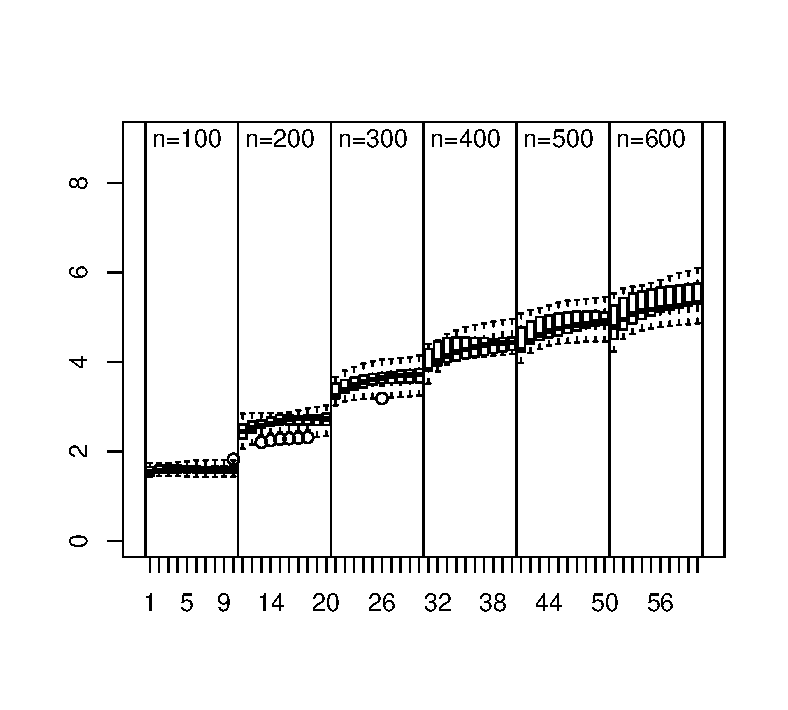
\includegraphics[scale = 0.7]{gabor_random_Y.pdf}
\caption{Confidence intervals for $I(\vec{g}_{Gabor}(X); Y)$, where $Y$ are subsamples of size $\{100, 200, \hdots, 600\}$ voxels
from V1.}
\end{figure}

Using the same voxel subsamples and parameters $k$, but now using a
reduced encoding model $\vec{g}_{reduced}$ with $p=681$,
we computed confidence intervals for
$I(\vec{g}_{reduced}(X); Y)$.

\begin{figure}
\centering
%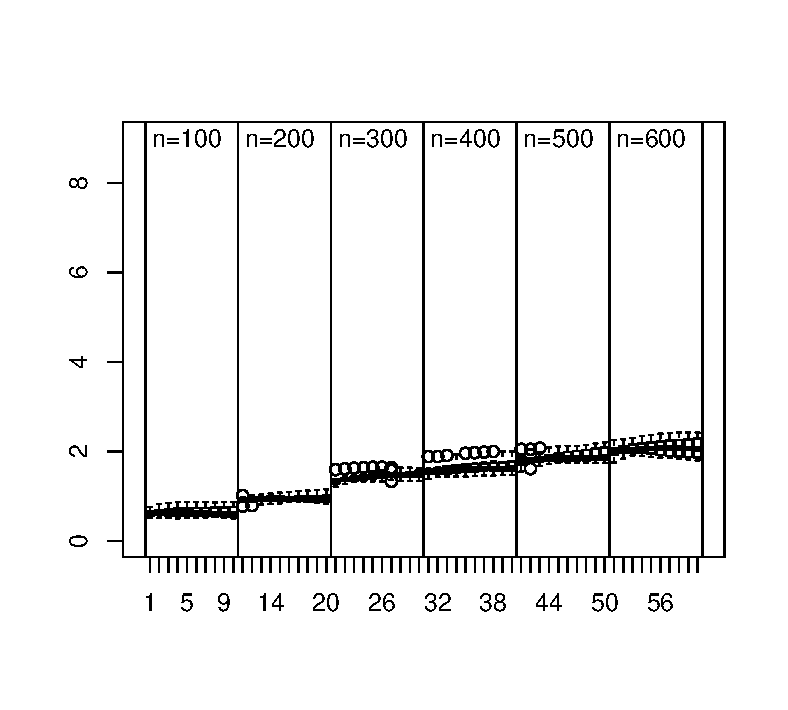
\includegraphics[scale = 0.7]{reduced_random_Y.pdf}
\caption{Confidence intervals for $I(\vec{g}_{reduced}(X); Y)$, where $Y$ are subsamples of size $\{100, 200, \hdots, 600\}$ voxels
from V1.}
\end{figure}



\section{Discussion}

Since the Bayes error is the large-sample
limit of the achieved classification error, a promising approach is to
perform classification using differently sized subsamples of the
training data, producing a plot of classification error versus sample
size--a ``learning curve.'' One can then extrapolate the learning
curve to estimate the Bayes error (Cortes et al. 1994.)However, much
work remains to develop rigorous methodology for estimating Bayes
error, and so we leave this first issue for future work.

We should keep in mind that the definition
of mutual information depends on the specific class of stimulus that
is of interest in the experiment.  The Bayes error itself depends on
the choices made by the experimenter in regards to the stimuli
exemplar chosen in the experiment, and the decision of how to
partition those exemplars in the classification task.  For example,
Nishimoto et al classified segments of a movie clips based on
activation patterns, but the definition of the classification task,
and the achievable classification performance, depends not only on the
particular move clips used in the experiment, but also the choice of
time interval used to define discrete classes: defining each class to
be a 1sec segment of movie results in more distinct classes and lower
classification accuracy than defining each class to be a 4sec segment
of movie. The Bayes error, and any estimate of mutual information
based on the Bayes error, would therefore be necessarily dependent on
the experimental parameters.


%% move somewhere
Estimating $e_{Bayes}$ is much more difficult in practice than
estimating $e_{gen}$; however, nonparametric estimators of $e_{Bayes}$
have been proposed in the literature.  Cover (1969) first noted that
the leave-one-out error of 1-nearest neighbor, $e_{1nn}$,
asymptotically bounds the Bayes error in the sense that
\[
\frac{1}{2}\E[e_{1nn}] \leq e_{Bayes} \leq \E[e_{1nn}].
\]
Later, Fukunaga and Kessel (1971) and Fralick and Scott (1971) both
proposed a consistent estimator of $e_{Bayes}$ using the test error
from kernel density estimation-based classifiers.  Fukunaga and
Hostetler 1975 improved on the density estimation approach by
estimating the generalization error directly, rather than using
empirical test error (hence reducing variance.)

%% move somewhere
Nevertheless, the convergence rates of nonparametric methods of Bayes
risk estimation are too slow to provide much assurance for their use
in high-dimensional problems.  On the other hand, the empirical
success of supervised learning approaches seems to justify a certain
optimism that at least one of the popular black-box methods (random
forests, neural networks, kernel SVM) can come close to the Bayes
error rate within realistic sample sizes.  Methods such as random
forests and neural networks are known to have \emph{universal
approximation} properties that guarantee consistent recovery of the
classification rule, given that the model complexity is scaled at an
appropriate rate as the sample size increases; but methods such as
kernel SVM have much more restrictive function classes and therefore
have no guarantee of being able to recover the Bayes error.  Yet, it
is seen in many learning tasks that the test error is very similar for
very different classification methods, some universal and some
non-universal, suggesting that the true signal lies in a
low-complexity function class which can be adequately approximated
using a variety of methods.  Empirical evidence for these phenomenon
are collected in studies on the learning curves of classifers,
beginning with Cortes 1994, and applied to specific applications by
Figueroa et al. 2012, Beleites et al. 2013.  We leave further
discussion of Bayes error estimation for future work; in the
theoretical portion of the current paper, we will simply leave
unspecified the method used to estimate Bayes error, and in our
simulation and real data examples, we will use an ad hoc approach for
estimating Bayes error from test error for the purpose of
demonstrating our method.


\section{Conclusions}

\begin{itemize}
\item We derive a relationship between average Bayes error (ABE) and mutual
  information (MI), motivating a novel estimator $\hat{I}_{LS}$.
\item Theory based on high dimensional, low SNR limit,
where \[\text{ABE} \leftrightarrow \text{MI}.\]
\item In ideal settings for supervised learning, ABE can be estimated
  effectively and $\hat{I}_{LS}$ can recover MI at much lower sample
  sizes than nonparametric methods.
\item In simulations, $\hat{I}_{LS}$ works better than Fano's
  inequality or the confusion matrix approach.
\end{itemize}

\section{References}
\begin{itemize}
\item Gastpar, M.  Gill, P.  Huth, A.  Theunissen, F. ``Anthropic Correction of Information Estimates and Its Application to Neural Coding.'' \emph{IEEE Trans. Info. Theory}, Vol 56 No 2, 2010.
\item  A. Borst and F. E. Theunissen, ``Information theory and neural coding''
Nature Neurosci., vol. 2, pp. 947?957, Nov. 1999.
\item L. Paninski, ``Estimation of entropy and mutual information,'' Neural
Comput., vol. 15, no. 6, pp. 1191?1253, 2003.
\item I. Nelken, G. Chechik, T. D. Mrsic-Flogel, A. J. King, and J. W. H.
Schnupp, ``Encoding stimulus information by spike numbers and mean
response time in primary auditory cortex,'' J. Comput. Neurosci., vol.
19, pp. 199?221, 2005.
\item Cover and Thomas.  Elements of information theory.
\item Muirhead.  Aspects of multivariate statistical theory.
\item van der Vaart.  Asymptotic statistics.
\end{itemize}
\end{document}





